\label{cap:proposal}
\chapter{Um Sistema de Recomendação Semântico baseado em conteúdo}

Desde de tempos o homem busca construir ferramentas e máquinas que facilitem, ampliem, sustem sua capacidade de trabalho e produção. Com o advento dos computadores e dos programas de máquina, o \textit{software} tornou-se essencial para a contínua demanda de problemas e desafios da crescente população global. Como avaliado por \cite{Sommerville2010},  o software não se restringe a propriedades materiais das leis da física ou por processos de manufatura. Por um lado, este fato simplifica a engenharia de software devido falta de restrições físicas, mas o torna complexo e de alto custo na realização de mudanças. Dessa forma, com a crescente quantidade de computadores e a diversidade de dispositivos, é cada vez mais relevante a qualidade de software.

O tema não é novo e já é levantado desde a década de sessenta, como na conferência NATO \citep{NR68} sobre problemas e desafios no desenvolvimento de software. A qualidade de software não somente aborda problemas do ponto de vista da coordenação do desenvolvimento, viabilizando a execução pelas máquinas, mas também estuda a importância da legibilidade a fim facilitar a manutenção e compreensão por humanos. Assim, é de suma importância documentar funcionalidades, decisões técnicas a serem utilizadas no processo do desenvolvimento de software, para que outros possam entender o trabalho que está sendo construído \citep{Pressman2009}.

Neste capítulo será apresentado os requisitos funcionais e não funcionais para um sistema de de recomendação semântico baseado em conteúdo. Serão discutida as tecnologias, comportamentos, modelos e arquiteturas utilizadas. Por fim, será demonstrado o funcionamento de um protótipo de um site para recomendações de filmes, implementando esse sistema.

\section{Requisitos}

Os requisitos de um sistema são descrições do que deve fazer, suas funcionalidades e serviços que restringem sua operação \citep{Sommerville2010}. Tais requisitos são uma reflexão das necessidades dos consumidores do sistema e definem um propósito específico, como cadastrar um usuário, encontrar produtos etc. Os requisitos de software, então, tratam-se de descobrir, analisar e documentar tais serviços e restrições para a operação do produto final. A descrição desses requisitos deve ser clara e objetiva, para apenas descrever o objetivo final da funcionalidade a ser desenvolvida.

Os requisitos de software são tradicionalmente classificados entre \textbf{funcionais} e \textbf{não funcionais}, para diferentes níveis de detalhamento e diferentes leitores.

\begin{itemize}
	\item{\textbf{Requisitos funcionais}: Descrevem o funcionamento do sistema, e para isso devem prover como o sistema deve reagir à entrada/saída assim como seus comportamentos em diferentes situações.}
	
	\item{\textbf{Requisitos não funcionais}: Devem estabelecer as restrições das funcionalidades e serviços oferecidos pelo sistema. São descritas caraterísticas gerais do sistema, como a usabilidade que não se referem a termos específicos como os requisitos funcionais. Comumente também são descritas questões que devem ser atendidas para a segurança e confiabilidade do sistema.}
\end{itemize}

Para cada requisito é utilizado um código para identificar a funcionalidade, assim facilitando referenciá-la durante o desenvolvimento. Nesta seção serão apresentados os requisitos funcionais e não funcionais para o desenvolvimento deste projeto. Para a descrição das funcionalidades optou-se por usar códigos com a sintaxe [RF0X] para requisitos funcionais e [RNF0X] para requisitos não funcionais. Junto ao código e a descrição do requisito foi adicionada a sua prioridade. As prioridades são classificadas em três categorias: a) \textbf{Essencial} para os que precisam ser implementados indispensavelmente, ou seja, são estritamente necessários para o funcionamento do sistema; b) \textbf{Importante} para os que são importantes para o funcionamento, mas não são cruciais; c) \textbf{Desejável} para os que não interferem diretamente nas funcionalidades básicas do sistema , embora relevantes, mas que podem ser deixados para ser implementados posteriormente.

\subsection{Requisitos funcionais}

A Tabela \ref{tab:req-funcionais} apresenta os requisitos funcionais do sistema.

\begin{table}[H]
	\label{tab:req-funcionais}
	\centering
	\caption{Requisitos funcionais do sistema.}
	\def\arraystretch{1.2} % padding da linhas da tabela
	\begin{tabular}{|m{1.2cm} | m{3cm} | m{7.2cm}| c | m{1.9cm}}
		\hline
		
		\multicolumn{1}{|c|}{\bfseries Código} & \multicolumn{1}{c|}{\bfseries Nome} & \multicolumn{1}{c|}{\bfseries Descrição} & \multicolumn{1}{c|}{\bfseries Prioridade} \\ \hline
		RF01	& Cadastrar usuário	& Realizar o cadastro de usuários para criação do seu perfil	& Essencial \\ \hline
		RF02	& Cadastrar usuário com o Facebook	& Permitir o cadastro de usuários utilizando sua conta do Facebook	& Importante \\ \hline
		RF03	& Fazer login/logout	& Usuários devem ser identificados permitindo a entrada e saída da aplicação	& Essencial \\ \hline
		RF04	& Fazer login pelo Facebook	& Permitir o login do usuário pelo Facebook	& Importante \\ \hline
		RF05	& Cadastrar filmes do usuário	& Usuários identificados podem cadastrar novos filmes no seu perfil	& Essencial \\ \hline
		RF06	& Visualizar filmes do usuário	& Usuários identificados podem visualizar os filmes cadastrados no seu perfil	& Essencial \\ \hline
		RF07	& Remover filmes do usuário	& Usuários identificados podem remover filmes cadastrados no seu perfil	& Essencial \\ \hline
		RF08	& Pesquisar filmes cadastrados	& Usuários identificados podem pesquisar filmes cadastrados na base do sistema	& Importante \\ \hline
		RF09	& Cadastrar filmes	& O sistema deve permitir a alimentação de filmes para a base dados	& Essencial \\ \hline
		RF010	& Edição de filmes	& O sistema deve permitir a edição de filmes alimentados para a base	& Essencial \\ \hline
		RF011	& Visualização de filmes recomendados	& O sistema deve ser capaz de criar uma lista de filmes recomendados, baseado nos filmes registrados do perfil do usuário	& Essencial \\ \hline
		RF012	& Coletar filmes do Facebook	& Usuários identificados devem podem importar filmes marcados no Facebook	& Importante \\ \hline
		RF013	& Visualizar informações do filme	& Usuários identificados devem ser capaz de visualização a informação de um filme específico, seja na lista de recomendações ou registrados no seu perfil	& Importante \\ \hline
	\end{tabular}
\end{table}

\subsection{Requisitos não funcionais}

A tabela \ref{tab:req-nao-funcionais} apresenta os requisitos não funcionais informando sua característica. Todos os requisitos apresentados são considerados essenciais.

\begin{table}[H]
	\label{tab:req-nao-funcionais}
	\centering
	\caption{Requisitos não funcionais do sistema.}
	\def\arraystretch{1.3} % padding da linhas da tabela
	\begin{tabular}{| m{1.3cm} | m{9.4cm}| c | m{2cm}}
		\hline
		\multicolumn{1}{|c|}{\bfseries Código} & \multicolumn{1}{c|}{\bfseries Descrição} & \multicolumn{1}{c|}{\bfseries Característica} \\ \hline
		RNF01	& O sistema deve ser fácil uso e dispensar prévio treinamento	& Usuabilidade \\ \hline
		RNF02	& O sistema deve ser simples de ser utilizado provendo informações e feedback de forma clara e objetiva	& Usuabilidade \\ \hline
		RNF03	& O sistema deve estar organizado de tal forma a não deixar o usuário confuso e ao mesmo tempo incentivar a sua exploração com interesse visual	& Usuabilidade \\ \hline
		RNF04	& O sistema deve ser capaz de atualizar as similaridades calculadas dos filmes em \textit{background}	& Funcionalidade \\ \hline
		RNF05	& O sistema deve prover uma metalinguagem para momentos em que o usuário deve aguardar o processamento de dados, tais como ícones, informativos etc.	& Usuabilidade \\ \hline
		RNF06	& O sistema deve possuir um desempenho adequado para que o cálculo da lista de filmes recomendados tenham o menor impacto de carregamento na navegação do usuário.	& Funcionalidade \\ \hline
		RNF07	& O sistema deve ser capaz de incluir novos filmes em \textit{background}	& Funcionalidade \\ \hline	
	\end{tabular}
\end{table}

\section{Arquitetura}

A arquitetura de software trata-se das estruturas e componentes, assim como as interações entre essas partes que irão compor o software do sistema. Para \cite{Perry1992} a arquitetura de software manifesta-se principalmente em partes do software do produto em relação a: 1) Requisitos para a determinação da informação, processamento e características que serão necessárias para o usuário e o sistema; 2) Arquitetura quando preocupa-se com a seleção de elementos, suas interações, e restrições necessárias para prover um \textit{framework} que satisfaça os requisitos; 3) Design quando está interessado na modularização e detalhamento do design dos elementos, algoritmos, procedimentos e tipos de dados que suportem a arquitetura e os requisitos; 4) Implementação quando preocupa-se com a representação de algoritmos, tipos de dados que satisfaçam a arquitetura, design e os requisitos.

Para a organização e estrutura deste projeto foi escolhida o padrão de arquitetura \ac{MVC}. O objetivo desse padrão é organizar o sistema em camadas em que cada uma seja responsável por funcionalidades específicas no fluxo entre o sistema e o usuário. Assim, o desenvolvimento e alterações podem ser realizadas de forma independente. No \ac{MVC} o sistema é estruturado em três camada que interagem entre si:

\begin{itemize}
	\item{\textbf{Model}: Camada da representação ou modelo para a manipulação dos dados da aplicação, sendo usado tanto na manipulação de elementos da interface como na persistência de dados.}
	
	\item{\textbf{View}: Camada da apresentação para o usuário, a interface. Envolve toda a parte de visualização de dados e interação com o sistema do ponto de vista do usuário.}
	
	\item{\textbf{Controller}: Camada que controla o fluxo das informações, validação, controle de acesso e comportamentos entre a \textit{view} e a \textit{model}.}
\end{itemize}

\section{Tecnologias}

Para o desenvolvimento do sistema foram escolhidas algumas tecnologias para arquitetura software, como linguagens de programação, \textit{framework} \ac{MVC}, processamento e banco dados, entre outras. A seguir serão apresentadas as tecnologias utilizadas.

\subsection{JAVA}

JAVA\footnote{https://www.java.com} é uma linguagem de programação de propósito genérico, desenvolvida originalmente por James Gosling na Sun Microsystems\footnote{ https://www.oracle.com/br/sun/index.html} em 1995. Atualmente a linguagem foi comprada pela Oracle Corporation\footnote{https://www.oracle.com}. As características em destaque da linguagem estão no fato de ser baseada em classes e orientada a objetos. A \ac{OOP} é um paradigma de programação que abstrai conceitos em objetos, que podem conter dados, campos e comportamentos nomeados de \textit{methods} \citep{Lewis2000}. 

Outra caraterística importante da linguagem trata-se da filosofia apresentada pelos desenvolvedores de “escreva uma vez, rode em qualquer lugar”. A filosofia trata-se da linguagem ser compilada por uma \ac{VM} possibilitando escrever um mesmo pedaço de código que possa ser portado para outra plataforma sem necessidade de alterá-lo, uma vez que cada \ac{VM} implementa as especificidades da nova plataforma abstraindo o acesso ao \ac{SO}.

A linguagem JAVA é usada em diversos sistemas e plataformas, com inúmeros propósitos, desde aplicações \textit{desktop}, pesquisa científica, desenvolvimento Web entre outros propósitos.

\subsection{Spring Boot}

Spring Boot\footnote{https://projects.spring.io/spring-boot/} é um projeto da 	Pivotal Software\footnote{https://pivotal.io} para facilitar o processo de configuração e publicação de aplicações e serviços providos pelo Spring\footnote{https://spring.io}, com baixo esforço e configuração. O \textit{Spring} é um framework \textit{open source}\footnote{Modelo de desenvolvimento que promove um licenciamento livre para o design ou esquematização  de um produto} que provê um compreensivo conjunto de modelos de configuração para aplicações JAVA. O elemento principal do \textit{Spring} é prover infraestrutura para aplicações oferecendo os seguintes principais recursos:

\begin{itemize}
	\item{\textbf{Inversão de Controle}: \ac{IOC}, também conhecido como \textit{dependency injection} é um princípio que as “dependências” devem ser supridas, injetadas por outro objeto. As dependências são objetos que serão usados como “serviços” para acessar suas funcionalidades, dentro dos \textit{containers} de \ac{IOC}. A injeção é a passagem da dependência para um objeto (o cliente) \citep{DependencyInjection2006}. O termo “inversão de controle” origina-se do fato que a criação de valores de classes externas ao objeto não deve ser realizada pelo próprio objeto mas, sim pelos \textit{containers} de \ac{IOC}.}
	
	\item{\textbf{Acesso a dados}: O framework possui diversas bibliotecas para o acesso a dados, tanto para bancos relacionais como não relacionais. Também é oferecido um sistema \ac{ORM} que trata-se de uma técnica para traduzir o formato de dados de um banco relacional para \ac{OOP}, facilitando sua manipulação.}
	
	\item{\textbf{Arquitetura MVC}: Fornece todo suporte para customizar e criar uma arquitetura \ac{MVC}.}
\end{itemize}

\subsection{HTML, CSS, Javascript}

O HTML\footnote{https://www.w3.org/html}, \ac{CSS}\footnote{https://www.w3.org/Style/CSS/} e JavaScript forma a principal pilha de tecnologias utilizadas na Web. O HTML é uma linguagem de marcação mantida pela \ac{W3C} para criação de páginas, originalmente desenvolvida por Tim-Berners-Lee \citep{Raggett1998}. O objetivo é a fácil construção e publicação de conteúdo no ambiente Web e consequentemente na \ac{WWW}. No \textit{Spring Boot} as páginas HTML podem ser escritas utilizando algum dos mecanismos de \textit{templates}, como o \textit{thymeleaf}. Uma das vantagens da utilização desses mecanismos é a herança de visualizações, assim como facilidade de interligar em manipular os dados passados pelo \textit{controller}.

O \ac{CSS} é uma linguagem para criar regras de estilização das páginas \ac{HTML}. O CSS cria ou altera um formato de apresentação (tamanho, cores, margens etc) de algum elemento do HTML, como blocos, parágrafos, imagens entre outros. Quanto ao JavaScript é uma linguagem de programação originalmente criada por Brendan Eich na Netscape Communications\footnote{ http://isp.netscape.com}. A linguagem é utilizada para controlar o comportamento de páginas HTML, oferecendo dinamicidade, podendo alterar elementos da página em tempo real.

\subsection{MySQL}

O MySQL\footnote{https://www.mysql.com} trata-se de um \ac{SGBD} que utiliza a linguagem \ac{SQL} para manipulação de dados guardados em um sistema de arquivos \citep{MySQLSGBD}. Originalmente desenvolvido por Michael Widenius em 1994, o seu foco é para o desenvolvimento de aplicações Web, embora tenha se popularizado para a maioria das plataformas existentes \citep{MySQLDevelopers}. Foi o banco de dados escolhido para a persistência de dados da aplicação, além de ser de fácil integração com o \textit{framework} \textit{Spring Boot}.

\subsection{Apache Jena}

Apache Jena\footnote{https://jena.apache.org} é um \textit{framework} \textit{open source} para Web Semântica, escrito na linguagem Java. A biblioteca provê uma \ac{API} que facilita a extração e criação de dados nos grafos  do \ac{RDF}, além de oferecer suporte para a linguagem de consulta \ac{SPARQL}. O objetivo da escolha dessa tecnologia para o projeto, é para facilitar a busca e navegação pelo grafo de entidades (\textit{resources}) no sistema da DBPedia\footnote{http://wiki.dbpedia.org} utilizando \ac{SPARQL}. Após o \ac{SR} extrair entidades das descrições do filme, essas serão buscadas no serviço da Web Semântica estendendo o conhecimento do recurso.

\subsection{Apache OpenNLP}

Apache OpenNLP\footnote{https://opennlp.apache.org} é um \textit{framework} \textit{open source} de aprendizado de máquina que é usado para processamento de \ac{NLP}. A biblioteca provê uma \ac{API} com serviços para geração de \textit{tokens}, sentenças, segmentação, reconhecimento de partes da fala, extração de entidade de nome, geração de \textit{chunks} (pedaços), entre outras tarefas do \ac{NLP}. A figura \ref{fig:nlp} mostra algumas das tarefas envolvidas no processamento de linguagem natural.

\begin{figure}
	\centering
	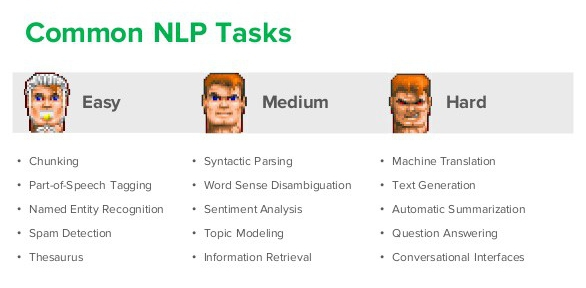
\includegraphics[scale=1]{imagens/nlp.jpg}
	\caption{Segmentação de tarefas no NLP. \citep{NLP2016}}
	\label{fig:nlp}
\end{figure}

No projeto essa tecnologia será utilizada para o \ac{NER} e extração de partes gramaticais presentes na descrição do filme, assim como a geração dos \textit{tokens}. O objetivo é que com essa biblioteca seja possível gerar \textit{tokens} com entidades encontradas, de nomes localizações, como também partes do texto de nomes próprios, substantivos e adjetivos.

\subsection{Apache Lucene}

Apache Lucene\footnote{https://lucene.apache.org} é um \textit{framework} \textit{open source} para sistemas de recuperação de informação e recomendação. O projeto oferece dois principais recursos: indexação e pesquisa de texto. Lucene é muito reconhecido por sua utilidade na implementação em mecanismos de buscas na Internet \citep{McCandless2010}. O projeto também é muito utilizado em sistemas de recomendação com implementação de diversos algoritmos para calcular a similaridade de documentos.
No projeto essa tecnologia será utilizada para tirar proveito dos algoritmos de similaridade, como o \textit{cossine similarity} (ver \ref{eq:cosine_sim}), possibilitando estender seu funcionamento e permitir integração com a biblioteca, facilitando o seu uso para outras pessoas e outros projetos.

\section{Funcionamento}

As tecnologias apresentadas anteriormente serão utilizadas para construir toda a arquitetura do sistema de recomendação. A proposta é criar uma recomendação baseada em conteúdo, e para este trabalho foi definido o domínio de filmes como exemplo de utilização. Sendo assim, o sistema possui algumas etapas de processamento para viabilizar a recomendação:

\begin{itemize}
	\item{\textbf{Coleta dos filmes}: Serão coletados dados dos filmes utilizando o projeto MovieLens\footnote{https://movielens.org} (ver \ref{ssec:dataModel}).}
	
	\item{\textbf{Coleta das preferências do usuário}: Serão coletados dados das preferências dos usuários, ou seja, os filmes de interesse. Nessa etapa poderá ser utilizada o perfil do Facebook\footnote{https://facebook.com} para obter tais dados.}
	
	\item{\textbf{Pré-processamento dos filmes}: Nessa etapa após a coleta dos filmes, os dados serão previamente processados para a geração de \textit{tokens} com \ac{NLP} analisando a descrição dos itens. Os dados gerados também serão expandidos analisando as entidades extraídas no \ac{NER} da sinopse do filme, com o serviço da DBPedia\footnote{http://wiki.dbpedia.org}. Após todos os processamentos os \textit{tokens} serão persistidos no banco de dados.}

	\item{\textbf{Cálculo da Similaridade}: Após a etapa de pré-processamento dos filmes, será realizado o cálculo da similaridade para todos os filmes da base dados utilizando uma similaridade do cosseno semanticamente estendida (ver \ref{ssec:recsysAlgo}). Os dados gerados serão persistidos no banco para viabilizar o desempenho da geração das recomendações.}
	
	\item{\textbf{Geração das recomendações}: Com as similaridades calculas e persistidas o sistema deverá gerar listas de filmes para recomendação (ver \ref{ssec:recsysAlgo}).}
	
	\item{\textbf{Apresentação dos resultados}: Apresentação dos resultados: Por fim o sistema apresentará os resultados das recomendações para o usuário.}		
\end{itemize}

\begin{figure}
	\centering
	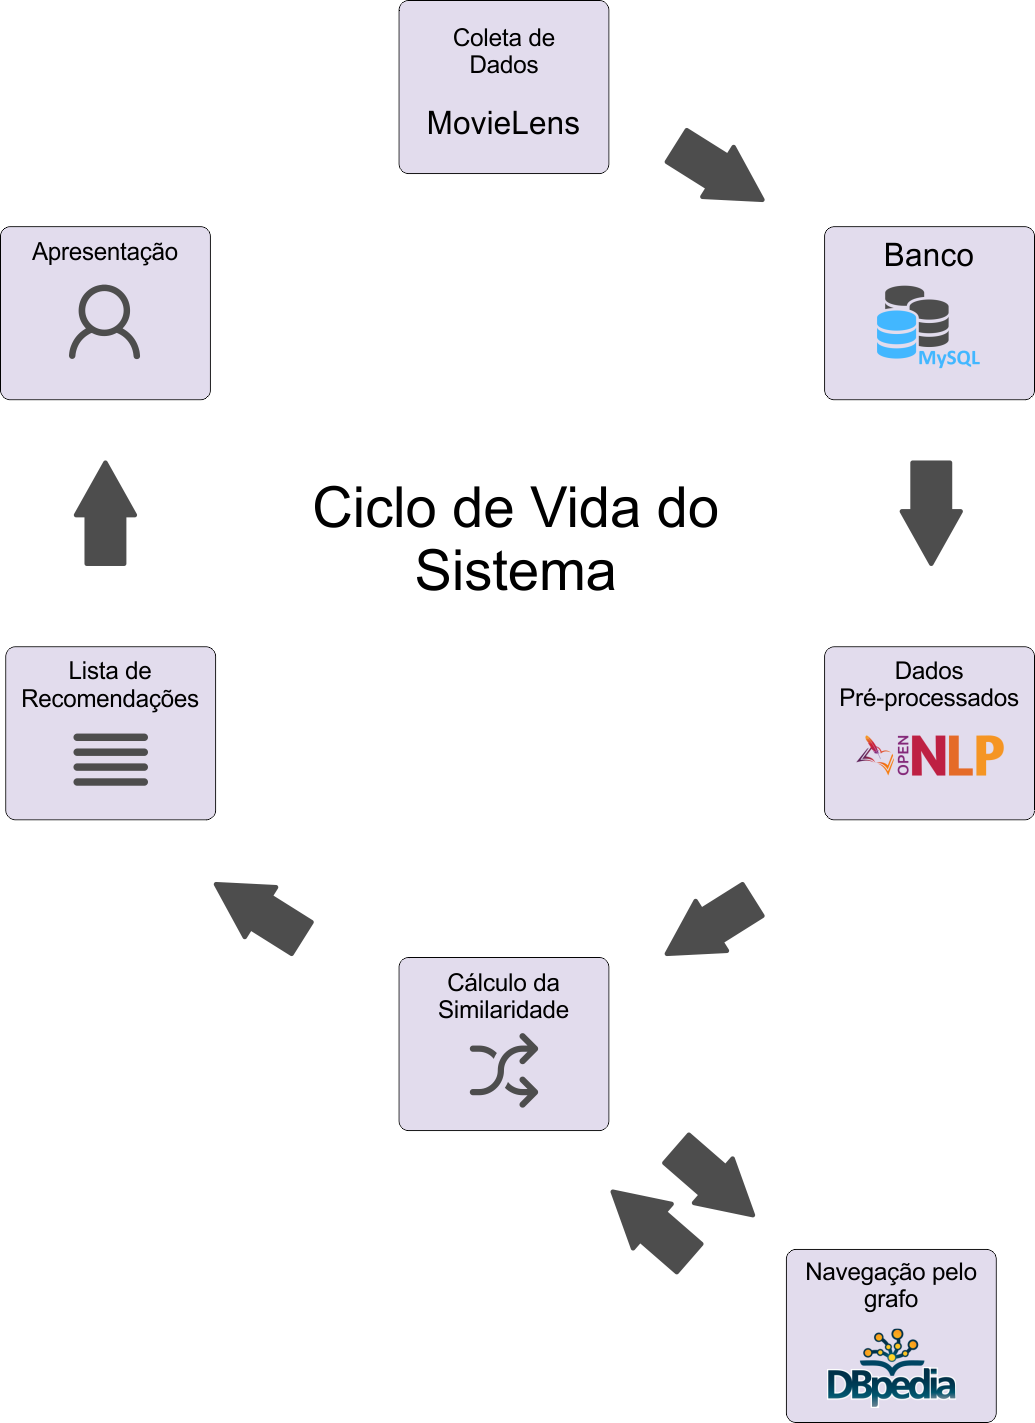
\includegraphics[scale=0.80]{imagens/recsys_fluxo.png}
	\caption{Fluxo das camadas do sistema de recomendação}
	\label{fig:recsys_fluxo}
\end{figure}

A \ref{fig:recsys_fluxo} mostra como esse fluxo de funcionalidades é operado por todo o sistema. A seguir será aprofundado mais algumas questões sobre a integração dessas camadas.

\subsection{Integração entre camadas}

\subsection{Modelo de dados}

\label{ssec:dataModel}

\subsection{Algoritmo de similaridade e recomendação}

\label{ssec:recsysAlgo}

\section{Sistema em ação}

\section{Sumário}
